\UseRawInputEncoding
\documentclass[10pt,twocolumn]{article}
\usepackage{iasted2}
%\usepackage{floatflt}
\usepackage[utf8]{inputenc}

\usepackage{times}
\usepackage[dvips]{graphicx}

\begin{document}

\date{}

\title{A BLIND AND ROBUST WATERMARKING SCHEME USING THE WAVELET TRANSFORM}

\author{Stewart I. Fraser \\
        Department of Engineering \\
        University of Aberdeen \\
        Aberdeen, AB24 3UE, UK \\
	%Tel: +44 1224 273830 \\
	%Fax: +44 1224 272497 \\
        Email: s.i.fraser@abdn.ac.uk 
        \and
        Alastair R. Allen \\
        Department of Engineering \\
        University of Aberdeen \\
        Aberdeen, AB24 3UE, UK \\
	%Tel: +44 1224 272501 \\
	%Fax: +44 1224 272497 \\
        Email: a.allen@abdn.ac.uk
}

\addtolength{\parskip}{0.4cm}

\maketitle
\thispagestyle{empty}

%%%% Replace with your abstract.
\noindent
{\bf\normalsize ABSTRACT}\newline {
A novel, quantization based method for watermarking digital images is presented here.
This new scheme utilises implicit visual masking by only inserting a watermark bit into 
wavelet coefficients of high magnitude. 
Also, this watermarking technique is blind (\emph{i.e.}, neither the original uncorrupted image
nor any side information is required in the recovery process) as well as being very 
computationally efficient.
This new watermarking algorithm combines and adapts various aspects from two existing watermarking methods.
%\cite{dugad, inoue}. 
Results show that the newly presented method improves upon both
of these existing techniques.
}
\vspace{2ex}


%%%% Replace with your keywords. 
\noindent
{\bf\normalsize KEY WORDS}\newline
{Watermarking Techniques, Digital Image Watermarking, Wavelet.}

\section{Introduction}
This paper introduces a new quantization based, blind watermarking algorithm operating within the wavelet domain. 
The motivation for this new algorithm was based upon various aspects from watermarking schemes presented by Dugad \emph{et al.}~\cite{dugad}
and Inoue \emph{et al.}~\cite{inoue}. The new algorithm improves upon the Dugad algorithm in that it can survive the same malicious attacks
whilst producing marked images of greater visual quality. An improvement is made upon the semi-blind Inoue scheme as the new method does not require
a file containing the positions of the marked coefficients (\emph{i.e.}, the new watermarking scheme is blind).




\section{Background}
Previously, Dugad \emph{et al.}~\cite{dugad} presented an additive watermarking method operating 
in the wavelet domain. A three level wavelet transform with a Daubechies 8-tap filter was used;
no watermark was inserted into the low-pass subband. 
Unlike some non-blind watermarking schemes \cite{cox, corvi},
this scheme allowed a watermark to be detected without requiring access
to the uncorrupted original image (\emph{i.e.}, it is a blind watermarking system).

The Dugad scheme also performed implicit visual masking as only wavelet coefficients
with a large enough magnitude were selected for watermark insertion.
Wavelet coefficients of large magnitude correspond
to regions of texture and edges within an image. This has the effect of making it difficult for a human 
viewer to perceive any degradation to an image marked via this scheme. Also, because wavelet coefficients
of large magnitude are perceptually significant, it is difficult to remove the watermark
without severely distorting the marked image.

The most novel aspect of this scheme was the introduction of
an \emph{image sized watermark} consisting of pseudo-random real numbers. 
However, only a few of these watermark values are added to the host image. Using an
image sized watermark \emph{fixes} the locations of the watermark values; thus, there is
no dependence on the ordering of significant coefficients in the correlation process for watermark detection.
This is advantageous as the correlation process is extremely sensitive to the ordering of significant coefficients and any
change in this ordering (via image manipulations) can result in a poor detector response.


Another watermaking algorithm operating upon significant coefficients within the wavelet domain (implemented via 5/3 taps
symmetric short kernel filters) was presented by Inoue \emph{et al.} \cite{inoue}.
This method takes a three level wavelet transform
of the image to be watermarked and
inserts the watermark into the 
detail coefficients at the coarsest scales (LH3, HL3 and HH3; the lowpass component LL3 is excluded).

The Inoue scheme is a quantization based watermarking technique which aims to modify 
wavelet coefficients of high magnitude thus embedding the watermark into 
edge and textured regions of an image. 
%The process for watermark insertion is as follows:
%\begin{enumerate}
%	\item Two thresholds, \emph{T1} and \emph{T2}, are selected and any one
%	of the subbands LH3, HL3 or HH3 is chosen. Next, 
%	significant coefficients $C_{k} (k=1,2,\cdot\cdot\cdot, N)$ satisfying 
%	$\mbox{\emph{T1}} < |C_{k}| < \mbox{\emph{T2}}$ are found. 
%	
%	\item A binary watermark is created, $W(k), k=1,2,\cdot\cdot\cdot, N$. 
%	
%	\item For $k = 1, 2, \cdot\cdot\cdot, N$, the watermark is embedded by 
%	modifying $|C_{k}|$ as follows: \\
%	If $W(k) = 1$ and $C_{k} > 0$, then $C_{k} = \mbox{\emph{T2}}$ \\
%	If $W(k) = 0$ and $C_{k} > 0$, then $C_{k} = \mbox{\emph{T1}}$ \\
%	If $W(k) = 1$ and $C_{k} < 0$, then $C_{k} = \mbox{\emph{-T2}}$ \\
%	If $W(k) = 0$ and $C_{k} < 0$, then $C_{k} = \mbox{\emph{-T1}}$
%
%	\item Save the embedded position, subband label and the 
%	two thresholds \emph{T1} and \emph{T2}.
%\end{enumerate}
%
%The following process details the steps involved for watermark detection:
%\begin{enumerate}
%	\item Using the subband label and the embedded position, the
%	recovered wavelet coefficients $C_{k}^{'}, k = 1,2,\cdot\cdot\cdot, N$ are obtained.
%
%	\item Check each $C_{k}^{'}$ individually: \\
%	If $|C_{k}^{'}| < (\mbox{\emph{T1}} + \mbox{\emph{T2}}) / 2$, then the
%	recovered watermark bit is a 0. \\
%	If $|C_{k}^{'}| \geq (\mbox{\emph{T1}} + \mbox{\emph{T2}}) / 2$, then the
%	recovered watermark bit is a 1. 
%\end{enumerate}
%-------------------------------------------------------------------------------------------
%Initially, two thresholds, \emph{T1} and \emph{T2}, are chosen and any one of the detail 
%subbbands from the third level of the wavelet transform are selected. Next, significant 
%coefficients, $C_{k}$, from the selected subbands are chosen according to $T1 < |C_{k}| < T2$.
%A binary watermark $W(k)$ is created and then embedded by modifying $|C_{k}|$ via: \\
%If $W(k) = 0$, $C_{k}^{new} = \mbox{sgn}(C_{k}) \mbox{\emph{ T1}}$ \\
%If $W(k) = 1$, $C_{k}^{new} = \mbox{sgn}(C_{k}) \mbox{\emph{ T2}}$ \\
%Finally, the embedded positions, subbabnd label and the two thresholds are saved.
%In order to detect the watermark, the detail subbands are re-established and the locations of 
%the marked coefficients, $C_{k}^{'}$, are ascertained from the saved position file. The watermark is then 
%decoded via: \\
%If $|C_{k}^{'}| < (\mbox{\emph{T1}} + \mbox{\emph{T2}}) / 2$, a 0 is recovered. \\
%If $|C_{k}^{'}| \geq (\mbox{\emph{T1}} + \mbox{\emph{T2}}) / 2$, a 1 is recovered.
%-------------------------------------------------------------------------------------------
The quantization process used by this scheme is very straightforward and simple to implement
as it requires a file to be saved detailing the locations of where the watermark bits were
embedded. It is thus a semi-blind scheme as opposed to a blind scheme.


\section{Advantages and disadvantages of the Dugad and Inoue watermarking algorithms}
The Dugad algorithm has three main advantages:
(1) It is a blind algorithm. 
(2) It incorporates implicit visual masking, thus, the watermark is inserted
into the perceptually significant areas of an image via a simple
and straightforward process.
(3) It uses an image sized watermark to 
negate the order dependence of significant coefficients in the detection process.

There are two main disadvantages to the Dugad algorithm:
(1) It embeds the watermark in an additive fashion.
This is a drawback as blind detectors for additive watermarking schemes must correlate the
possibly watermarked image coefficients with the known
watermark in order to determine if the image has or has not 
been marked. Thus, the image itself must be treated as noise 
which makes detection of the watermark exceedingly difficult \cite{meerwald}.
In order to overcome this, it is necessary to correlate a very high number
of coefficients (which in turn requires the watermark to be embedded into many
image coefficients at the insertion stage). This has the effect of 
increasing the amount of degradation
to the marked image.
(2) The detector can only tell if the watermark is
present or absent. It cannot recover the actual watermark.

The Inoue algorithm has three main advantages:
(1) It uses a scalar quantization process to embed the 
watermark. This is an advantage as quantization
based watermarking schemes do not suffer from host image
interference \cite{meerwald} (unlike additive watermarking schemes).	
Hence, detectors from quantization
based watermarking techniques can operate successfully using a much smaller
watermark than is possible for additive schemes. This has the knock-on effect
of reducing the amount of degradation suffered 
by a marked image.
(2) The detector can recover the binary watermark
sequence thereby allowing the user to see it.
(3) Like the Dugad scheme, the watermark is embedded into perceptually significant coefficients.

The Inoue algorithm has one main disadvantage:
(1) It is a semi-blind algorithm. This is because it
requires a file containing the locations of where the watermark
was embedded in order for the detector to work. 



%\section{Advantages and disadvantages of the Dugad and Inoue watermarking algorithms}
%\underline{{\bf Advantages of the Dugad algorithm:}} 
%\begin{itemize} 
%	\item It is a blind algorithm. 
%	%Only the seed value for regenerating the image sized watermark and 
%	%the threshold value \emph{T2} are needed to detect the watermark.
%	\item It uses implicit visual masking. Thus, the watermark is inserted
%	into the perceptually significant areas of an image via a simple
%	and straightforward process.
%	\item It uses an image sized watermark to 
%	negate the order dependence of significant coefficients in the detection process.
%\end{itemize}
%%\newpage
%\underline{{\bf Disadvantages of the Dugad algorithm:}}
%\begin{itemize}
%	\item It embeds the watermark in an additive fashion.
%	This is a drawback as blind detectors for additive watermarking schemes must correlate the
%	possibly watermarked image coefficients with the known
%	watermark in order to determine if the image has or has not 
%	been marked. Thus, the image itself must be treated as noise 
%	which makes detection of the watermark exceedingly difficult \cite{meerwald}.
%	In order to overcome this, it is necessary to correlate a very high number
%	of coefficients (which in turn requires the watermark to be embedded into many
%	image coefficients at the insertion stage). This has the effect of 
%	%decreasing the robustness of the watermarking scheme as well as
%	increasing the amount of degradation
%	to the marked image.
%	\item The detector can only tell if the watermark is
%	present or absent. It cannot recover the actual watermark.
%\end{itemize}
%\underline{{\bf Advantages of the Inoue algorithm:}} 
%\begin{itemize}
%	\item It uses a scalar quantization process to embed the 
%	watermark. This is an advantage as quantization
%	based watermark schemes do not suffer from host image
%	interference \cite{meerwald} (unlike additive watermarking schemes).	
%	Hence, detectors from quantization
%        based watermarking techniques can operate successfully using a much smaller
%	watermark than is possible for additive schemes. This has the knock-on effect
%	%of increasing robustness as well as 
%	of reducing the amount of degradation suffered 
%	by a marked image.
%	\item The detector can recover the binary watermark
%	sequence thereby allowing the user to see it.
%	\item Like the Dugad scheme, the watermark is embedded into perceptually significant coefficients.
%\end{itemize}
%\underline{{\bf Disadvantages of the Inoue algorithm:}} 
%\begin{itemize}
%        \item It is a semi-blind algorithm. This is because it
%	requires a file containing the locations of where the watermark
%	was embedded in order for the detector to work. 
%\end{itemize}


\section{A new approach}
%The Dugad and Inoue schemes are quite similar in that they both use two threshold values and
%they both operate in the wavelet domain. 
%By using two threshold values, the lengths of watermarks inserted into different
%types of images (smooth or textured) will vary. 
%Nevertheless, as previously pointed out, both have
%good and bad points. 
%However, combining both schemes in a judicious fashion can result in 
%a new method which shares the advantages of both schemes whilst discarding most of the disadvantages.
It is possible to share the advantages of both the Dugad and Inoue watermarking schemes
whilst removing most of the disadvantages.
This can be achieved by using Dugad's idea of an image sized watermark in conjunction with
adapted versions of Inoue's scalar quantization insertion/detection techniques.
The resultant watermarking system will be blind and quantization based. It will 
employ a watermark equal in size to the detail subbands from the coarsest wavelet level
and only perceptually significant coefficients will be used to embed watermark bits.
%The resulting algorithm then has the following features:
%\begin{itemize}
% 	\item It is completely blind (unlike the semi-blind scheme of Inoue).
%	\item It is a quantization based technique (unlike the Dugad method).
%	This allows:
%	\begin{itemize}
%		\item The user to view a recovered watermark.
%		\item Less coefficients to be marked thereby producing watermarked images 
%		with very little degradation.  
%		%This is possible as detectors for quantization 
%		%based schemes do not suffer from host image noise (unlike additive schemes).
%		%Thus, they do not require a large amount of coefficients to be marked 
%		%in order for reliable detection.
%	\end{itemize}
%	\item It employs implicit visual masking as only wavelet coefficients\footnote{from
%	the detail subbands, the low-pass subband is not used for watermark insertion.}
%	of high magnitude at the third level are considered for watermark embedding.
%	These are perceptually significant coefficients thus making the scheme robust.
%	%Also, these coefficients correspond to edge and texture regions of images and are
%	%thus best suited for creating watermarked images that do not appear degraded 
%	%to human viewers.
%	\item 
%	%It uses an image sized watermark.
%	It uses a watermark the same size as the third level subband images (as opposed
%	to Dugad's method of an image sized watermark). This is done as only the third
%	level wavelet coefficients are to be marked (hence creating an image sized watermark
%	would be redundant). 
%	This third level subband sized watermark removes the need for 
%	a position file in the recovery process (thereby improving upon the Inoue scheme). 
%\end{itemize}
In summary, this new technique improves upon the Dugad method by using a 
quantize and replace insertion process (rather than an additive insertion process).
Thus, for comparable robustness performance, the new method will produce watermarked images
with less degradation than the Dugad scheme.
It improves upon the Inoue scheme
by having no need for a position file in the recovery process.

\begin{figure*}[!t]
	\begin{center}
		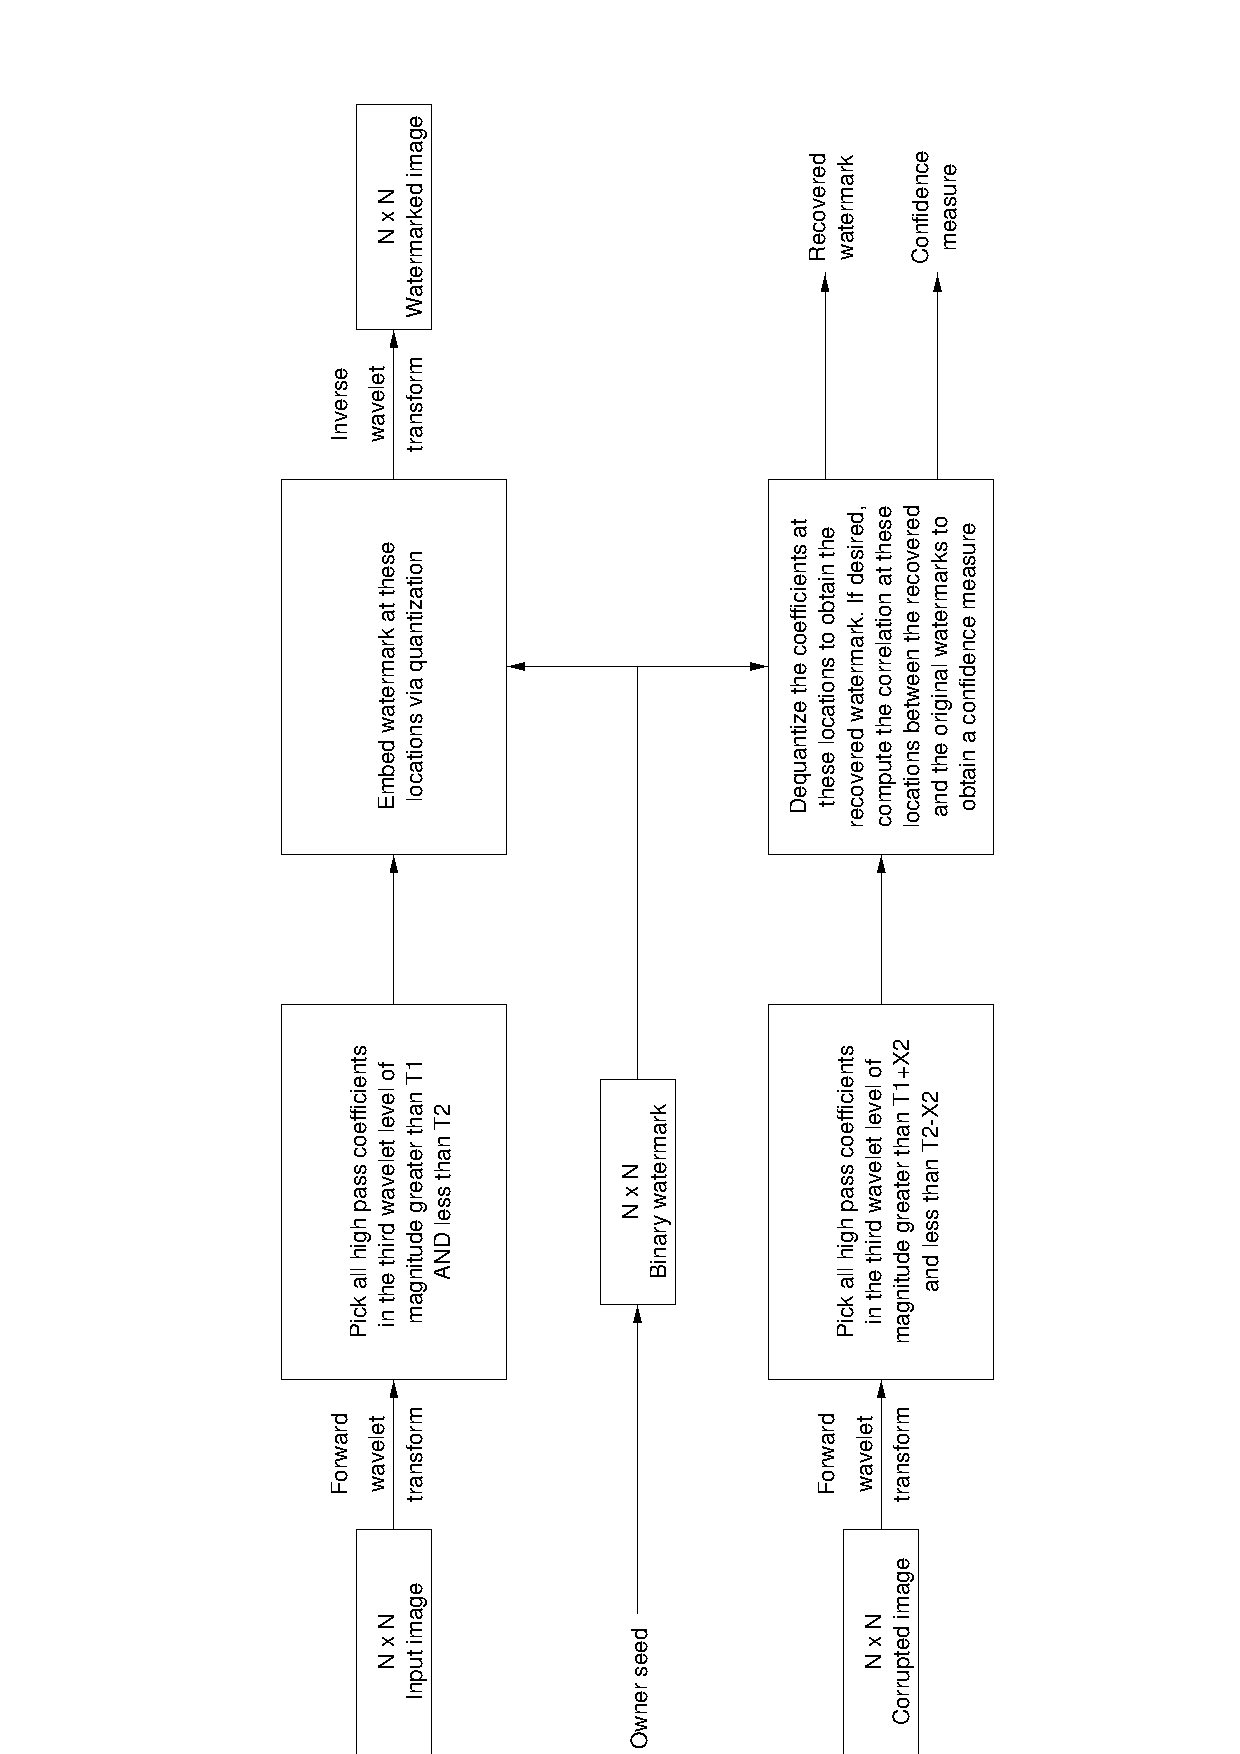
\includegraphics[height=6cm,width=13cm]{../pics/novelAlg3.pstex}
	\end{center}
	\caption{The blind quantization based watermarking scheme. The top part shows
	the insertion process whereas the bottom part shows the detection process.}
	%Note that DWT is the Discrete Wavelet Transform and the IDWT is the Inverse Discrete Wavelet Transform.}
	\label{novelAlg}
\end{figure*}


%\section{Implementation}
A flow diagram detailing the necessary steps is shown in Figure \ref{novelAlg}.
Note that the quantization and dequantization steps are explained in more
detail in Sections \ref{sub:embed} and \ref{subsec:det}, respectively.
\subsection{Embedding}
\label{sub:embed}
The watermark embedding process transforms the host image into the wavelet domain (the
current implementation uses Daubechies wavelets of length 4). Next, all the coefficients in the third
wavelet level (excluding the LL subband) with magnitude
greater than \emph{T1} and magnitude less than \emph{T2} are selected. 
A binary watermark
the same size as the 
%host image 
entire third level of the wavelet transform
is created using a secret key (which is a seed to a random
number generator). 

The selected wavelet coefficients are then quantized 
in order to embed a watermark bit. 
The value that the selected coefficients are quantized to depends upon
whether they are embedding a 1 or a 0. A selected wavelet coefficient, $w^{s}_{ij}$,
will embed a 1 if the value in the watermark file at the same location, $x_{ij}$, is 1.
Alternatively, $w^{s}_{ij}$ will embed a 0 if $x_{ij}$ is 0.
%The quantization method is similar to that used by Inoue: \\
Thus, the adapted Inoue quantization method for watermark insertion is: \\
%If $x_{ij} = 1$ and $w^{s}_{ij} > 0$, then $w^{s}_{ij} = \mbox{\emph{T2 - X1}}$, \\
%If $x_{ij} = 0$ and $w^{s}_{ij} > 0$, then $w^{s}_{ij} = \mbox{\emph{T1 + X1}}$, \\
%If $x_{ij} = 1$ and $w^{s}_{ij} < 0$, then $w^{s}_{ij} = \mbox{\emph{-T2 + X1}}$ \\
%If $x_{ij} = 0$ and $w^{s}_{ij} < 0$, then $w^{s}_{ij} = \mbox{\emph{-T1 - X1}}$ \\
If $x_{ij} = 0$ then $w^{s}_{ij} = \mbox{sgn}(w^{s}_{ij})(\mbox{\emph{T1 + X1}})$ \\
If $x_{ij} = 1$ then $w^{s}_{ij} = \mbox{sgn}(w^{s}_{ij})(\mbox{\emph{ T2 - X1}})$ \\
The \emph{X1} parameter narrows the range between the two quantization values of \emph{T1}
and \emph{T2} in order
to aid robust oblivious detection (see Section \ref{subsec:det}).

After all the selected coefficients have been quantized, the inverse wavelet 
transform is applied to all the wavelet coefficients and the watermarked image
is obtained.


\subsection{Detection}
\label{subsec:det}
For oblivious detection, the wavelet transform of a possibly corrupted
watermark image is taken. Then all the wavelet coefficients of magnitude greater than
or equal to \emph{T1 + X2} and less than or equal to \emph{T2 - X2} are selected;
these shall be denoted via $w'^{s}_{ij}$.

Note that \emph{X2} should be less than \emph{X1}. 
%Figure \ref{newQuant} shows the need to introduce
%the new parameters of \emph{X1} and \emph{X2}. 
In the insertion process, all wavelet coefficients
with a magnitude greater than \emph{T1} and less than \emph{T2} are selected and then quantized to
either \emph{T1 + X1} or \emph{T2 - X1}. In the recovery process, all the wavelet coefficients
of magnitude greater than or equal to \emph{T1 + X2} and less than or equal to \emph{T2 - X2} are 
selected to be dequantized.
This helps ensure that all the marked coefficients are recovered and dequantized after
being attacked. Also, 
unmarked coefficients are unlikely to drift into the range of selected coefficients
after an attack. The introduction of the \emph{X1} and \emph{X2} parameters to the watermarking algorithm
gives a degree of tolerance to the system against attacks, \emph{i.e.}, they collaborate to give a noise margin.

\begin{table*}[!t]
\begin{center}
%\renewcommand{\baselinestretch}{2}
\begin{scriptsize}
\begin{tabular}{|p{2.75cm}|c|c|c|c|c|c|c|c|c|c|} \hline
%\begin{tabular}{|c|c|c|p{0.5cm}|p{0.5cm}|p{0.5cm}|p{0.5cm}|c|c|p{0.5cm}|p{0.5cm}|p{0.5cm}|p{0.5cm}|} \hline
& No &\multicolumn{3}{|c|}{JPEG} & \multicolumn{2}{|c|}{Median filter} 
	& \multicolumn{2}{|c|}{Noise addition} & Cropp- & Half \\ \cline{3-9} %\cline{12-13}   
	%&\multicolumn{2}{|c|}{Mean filter} 
& attack & Q5 & Q10 & Q15 & $3 \times 3$ & $5 \times 5$ 
	& Gaussian & Impulse & ing & sizing \\ \hline   %& $3 \times 3$ & $5 \times 5$ \\ \hline
Average correlation & 32.43 & 12.17 & 17.83 & 20.85 & 25.16 & 17.74 & 14.57 & 12.96 & 22.04 & 16.16 \\ \hline %& 27.52 & 21.12   \\ \hline
Average detector threshold & 9.00 & 9.12 & 9.20 & 9.16 & 9.26 & 9.38 & 7.77 & 8.04 & 9.83 & 8.51 \\ \hline %& 9.23 & 9.27 \\ \hline
Average WM length in & 2552 & 2552 & 2552 & 2552 & 2552 & 2552 & 2552 & 2552 & 2552 & 2552 \\ \hline %& 2552 & 2552 \\ \hline
Average WM length out & 1788 & 1534 & 1560 & 1617 & 1274 & 933 & 3151 & 3920 & 1016 & 1957 \\ \hline %& 1016 & 615 \\ \hline
Average PSNR (dB) & 37.38 & 37.40 & 37.50 & 37.42 & 37.29 & 37.52 & 37.24 & 37.43 & 37.39 & 37.27 \\ \hline %& 37.42 & 37.25 \\ \hline
%wPSNR (dB) & & & & & & & & & & & & \\ \hline
Average TPE & 0.014 & 0.014& 0.014& 0.014& 0.014& 0.014& 0.014& 0.014& 0.014& 0.014\\ \hline %& 0.014& 0.014\\ \hline
Failures (false negatives)& 0 & 5 & 1 & 0 & 0 & 0 & 0 & 0 & 0 & 0 \\ \hline %& 0 & 0 \\ \hline
\end{tabular}
\end{scriptsize}
%\renewcommand{\baselinestretch}{2}
\end{center}
\caption{Dugad results. \emph{T1} = 40, \emph{T2} = 50 and $\alpha$ = 0.2. Each test was run
	30 times upon the Lena image with a different seed and the average result was then calculated.
	Note that WM refers to WaterMark.}
\label{dugResults}
\end{table*}
A watermark
bit is decoded for each of the selected wavelet coefficients via the same process
described by Inoue: \\
If $|w'^{s}_{ij}| < (\mbox{\emph{T1}} + \mbox{\emph{T2}}) / 2$, a 0 bit is recovered \\
If $|w'^{s}_{ij}| \geq (\mbox{\emph{T1}} + \mbox{\emph{T2}}) / 2$, a 1 bit is recovered \\
The recovered watermark is then correlated with the original copy of the
watermark file (obtained via the secret key) only in the 
locations of the selected coefficients. This allows a confidence measure
to be ascertained for the presence or non-presence of a watermark in an 
image.

\section{Results}
This section outlines the results obtained by Dugad's scheme and the newly 
proposed scheme. It is the aim of the new scheme to be as robust as
the Dugad scheme without degrading the marked images to the same extent. 
This newly proposed blind scheme improves upon the semi-blind Inoue scheme
as it does not require a file containing the locations of the coefficients that were marked.

In order to measure the degradation suffered by host images after watermark insertion, the
Peak Signal to Noise Ratio (PSNR) metric and the Watson Metric \cite{watsonDCT, mayache} are used.
The Watson Metric computes the Total Perceptual Error (TPE)
which is an image quality metric based upon the Human Visual System (HVS).
It takes contrast sensitivity,
luminance masking and contrast masking into account when calculating 
a perceptual error value (unlike the PSNR, which merely measures the differences
between pixels without considering the HVS). The higher the TPE value, the more degraded an
image would appear to a human viewer.
The Checkmark package \cite{ChkMrk:pereira} (\emph{WatsonMetric.m}) was used to determine the TPE.

For all the tests in this paper, MATLAB
6.0.0.88 Release 12 was used. JPEG compression was carried out via the \emph{imwrite}
function which uses the Independent JPEG Group's (www.ijg.org) LIBJPEG library.  
All tests were performed upon an 8-bit (greyscale), $256 \times 256$, Lena image.

%Because this new scheme has the advantageous property of not requiring a
%position file in the recovery process, it cannot match the robustness
%performance presented by Inoue. However, this is to be expected as 
%non-blind and semi-blind watermarking schemes gain robustness via
%the secret information (uncorrupt original images, position files, \emph{etc}.)
%that the detectors require.

\subsection{Dugad's results}
\label{sec:dugRes}
%In Dugad's paper, the response of the detector to various attacks was presented.
%However, a measure of the image degradation was not reported (only a watermarked
%image was presented for visual inspection). Thus, in order to ascertain a measure
%of the image degradation suffered due to Dugad's scheme, it is necessary to 
%encode the scheme to reproduce the same results and then obtain a quantitative
%measure of the image degradation. In order to achieve this, the same image 
%that Dugad used will be used here; \emph{i.e.}, Lena (8-bit greyscale, $256 \times 256$). Both
%the Peak Signal to Noise Ratio (PSNR) and the Total Perceptual Error (TPE) between the original and
%the watermarked images are computed. 
%%%%%%%%%%%%%%%%%%%%%%%%%%%%%%%%%%%%%%%%%%%%%%%%%%%%%%%%%%%%%%%%%%%%%%%%%%%%%%%%%%%%%%%%%%%%%%%%%%%%%%%%%
%In Dugad's paper, a quantitative measure of the image degradation suffered after inserting a watermark was not
%reported (only a watermarked image was presented for visual inspection). 
%Thus, it was necessary to encode the Dugad algorithm to determine the amount of image degradation 
%suffered by watermark insertion\footnote{the same algorithmic parameters used by Dugad are used here, namely: \emph{T1} = 40,
%\emph{T2} = 50 and $\alpha=0.2$}. 
%Like in Dugad's paper,
%an 8-bit greyscale $256\times 256$ Lena image was used as the host for the watermark. 
%Table \ref{dugResults} outlines the robustness of the Dugad algorithm to various attacks as well as
%stating the image degradation suffered due to watermark insertion.
The Dugad algorithm was encoded and the following parameters were set: \emph{T1} = 40, \emph{T2} = 50
and $\alpha=0.2$ (the same parameters that were used in the Dugad paper). 
The watermarked image was then attacked with 
JPEG quality 5 (Q5), quality 10 (Q10) and quality 15 (Q15), 
median filter with kernel size $3 \times 3$ and $5 \times 5$, 
Gaussian noise addition ($\sigma^{2}=375$),
impulse noise (normalised density of 0.015),
cropping (from rows 60 to 190 and from columns 60 to 190) and
half-sizing.
Also, each of the attacks was performed 30 times upon each watermarked Lena image (using a different seed each time)
and then averaged. 
%This is in contrast to the Dugad paper which only used a single seed value of 100 for each test.

%Another consideration 
%to note about the results presented by Dugad is that
%only a single seed value (of 100) was used 
%for each attack.
%This is important as the
%random number generator used by Dugad will almost certainly 
%be different from 
%the one used here. In order to accommodate this, the same attack was performed
%30 times upon the Lena image watermarked using a different seed each time. The 
%average of the results was then taken and are shown in Table \ref{dugResults}.
%%Figure \ref{lenaDugOurs}(a) shows the Lena image watermarked via Dugad's scheme.


%As well as the non-attacked case, the following attacks were performed here:
%JPEG quality 5 \underline{(Q5)}, quality 10 (Q10) and quality 15 (Q15),
%median filter with kernel size $3 \times 3$ and \underline{$5 \times 5$},
%\underline{Gaussian noise addition} ($\sigma^{2}=375$),
%impulse noise (normalised density of 0.015),
%\underline{cropping} (from rows 60 to 190 and from columns 60 to 190) and
%\underline{half-sizing}.
%Note that more attacks were performed here than were performed in the Dugad paper 
%(which are underlined).
%Also, each of the attacks was performed 30 times upon each watermarked Lena image (using a different seed each time) 
%and then averaged. This is in contrast to the Dugad paper which only used a single seed value of 100 for each test.

%Note that the results presented in Table \ref{dugResults} are virtually identicle to that presented in the 
%Dugad paper. The only variation is the Gaussian noise attack result. In the Dugad paper, it was stated that
%Gaussian noise attacks with $\sigma^{2}=600$ could be survived with an approximate correlation value of 15.
%However, the results here show that for a correlation value of approximately 15, only Gaussian noise attacks
%with $\sigma^{2}=375$ could be withstood. This rogue result may be attributed to only a single test being 
%carried out by Dugad as opposed to the 30 tests being carried out here.

%Also, it is noted that the average correlation value of approximately 12 was achieved for JPEG quality 5 attacks 
%(the same result reported by Dugad).
%However, in reaching this average value, 5 out of 30 false negative readings were obtained. Hence, it cannot be
%said that the Dugad scheme (operating under the parameters used here) is robust against JPEG quality 5 attacks.
%This conclusion can be extended to JPEG quality 10 attacks too.




Further confirmation of the quantitative image quality values was obtained by 
using a secondary implementation of the Dugad algorithm available from 
\cite{meerwald}. For thirty trials, each with a different seed value,
the average PSNR was 37.94 dB and the average TPE was 0.013 
(using a block size of $16 \times 16$).
This helps to validate the results in Table
\ref{dugResults}, where the average (from 300 tests; 30 trials for each of the 10 attacks)
PSNR is 37.38 dB and the
average TPE is 0.014 (again using blocks of size $16 \times 16$).


On average, it can be seen that the Dugad scheme is surviving all the attacks.
However, for the JPEG quality 5 and 10 attacks, the watermark was not 
always detected (\emph{i.e.}, a false negative reading was recorded).
It can therefore be said that the Dugad scheme is reliable only for 
JPEG attacks of quality 15 and higher.


\begin{table*}[!t]
\begin{center}
%\renewcommand{\baselinestretch}{2}
\begin{scriptsize}
%\begin{tabular}{|p{2.75cm}|c|c|p{0.65cm}|p{0.65cm}|p{0.65cm}|p{0.65cm}|p{0.9cm}|p{0.9cm}|p{0.65cm}|p{0.65cm}|} \hline
\begin{tabular}{|p{2.75cm}|c|c|p{0.9cm}|p{0.9cm}|p{0.9cm}|p{0.9cm}|p{0.9cm}|p{0.9cm}|p{0.9cm}|p{0.9cm}|} \hline

& No &\multicolumn{3}{|c|}{JPEG} & \multicolumn{2}{|c|}{Median filter} 
	& \multicolumn{2}{|c|}{Noise addition} & Cropp- & Half \\ \cline{3-9} %\cline{12-13} 
	%&\multicolumn{2}{|c|}{Mean filter} \\ \cline{3-9} \cline{12-13}
& attack  & Q5 & Q10 & Q15 & $3 \times 3$ & $5 \times 5$ 
	& Gaussian & Impulse & ing & sizing \\ \hline %& $3 \times 3$ & $5 \times 5$ \\ \hline
Average NC & 1.00 & 0.20 & 0.62& 0.84 & 0.89& 0.30& 0.52& 0.64& 0.53& 0.51\\ \hline %& 0.51& -0.26\\ \hline
Detector threshold chosen & 0.40 & 0.40 & 0.40 & 0.40 & 0.40 & 0.40 & 0.40 & 0.40 & 0.40 & 0.40   \\ \hline
Average WM length in & 188 & 188 & 188 & 188 & 188 & 188 & 188 & 188 & 188 & 188 \\ \hline %& 188 & 188 \\ \hline
Average WM length out & 188 & 153 & 165 & 170 & 168 & 163& 159& 154& 72& 142\\ \hline %& 151& 112\\ \hline
Average PSNR (dB) &  43.04 & 43.01 & 43.32 & 43.07 & 43.13 & 43.14& 43.15& 43.07& 43.01& 42.85\\ \hline %& 43.13& 43.02\\ \hline
Average TPE & 0.006 & 0.005 & 0.005 & 0.005 & 0.005& 0.005& 0.005& 0.006& 0.005& 0.005\\ \hline %& 0.005& 0.005\\ \hline \hline
%$ \times 10^{}$
\end{tabular}
\end{scriptsize}
%\renewcommand{\baselinestretch}{2}
\end{center}
\caption{Results for the new scheme (with \emph{T1} = 115, \emph{T2} = 200, \emph{X1} = 20 and \emph{X2} = 10). Each test was run
	30 times upon the Lena image with a different seed and the average results were then calculated.}
	%Note that WM refers to WaterMark.}
\label{ourResults}
\end{table*}
\begin{table*}
\begin{center}
%\renewcommand{\baselinestretch}{2}
\begin{scriptsize}
%\begin{tabular}{|p{1.9cm}|p{1.1cm}|p{0.65cm}|p{0.65cm}|p{0.65cm}|p{0.65cm}|p{0.65cm}|p{0.9cm}|p{0.9cm}|p{0.65cm}|p{0.65cm}|} \hline
\begin{tabular}{|p{3.5cm}|p{1.1cm}|p{0.9cm}|p{0.9cm}|p{0.9cm}|p{0.9cm}|p{0.9cm}|p{0.9cm}|p{0.9cm}|p{0.9cm}|p{0.9cm}|} \hline
& No &\multicolumn{3}{|c|}{JPEG} & \multicolumn{2}{|c|}{Median filter} 
	& \multicolumn{2}{|c|}{Noise addition} & Cropp- & Half \\ \cline{3-9} %\cline{12-13} 
	%&\multicolumn{2}{|c|}{Mean filter} \\ \cline{3-9} \cline{12-13}
& attack  & Q5 & Q10 & Q15 & $3 \times 3$ & $5 \times 5$ 
	& Gaussian & Impulse & ing & sizing \\ \hline %& $3 \times 3$ & $5 \times 5$ \\ \hline

Minimum NC & 1.00 & 0.03 & 0.56& 0.78& 0.82& 0.23& 0.45& 0.62& 0.43& 0.42\\ \hline %& 0.39& -0.36\\ \hline
Minimum length of recovered WM& 188 & 144 & 159 & 161& 160& 157& 155& 139& 69& 128\\ \hline %& 144& 122\\ \hline
%Highest Individual Pfp & - & 0.37 & $3.25 \times 10^{-14}$& $ 9.38\times10^{-27}$
%	& $ 1.50\times10^{-31}$& $ 2.19\times10^{-3}$
%	& $ 1.52\times10^{-8}$& $ 3.34\times10^{-18}$
%	& $ 7.58\times10^{-4}$& $ 3.62\times10^{-7}$\\ \hline 
%	%& $ 2.26\times10^{-7}$& 1.00\\ \hline
Worst case Pfp (using minimum NC and minimum length)& $<1.00\times10^{-50}$& $5.30\times10^{-1}$  & $3.58\times10^{-13}$ &$ 1.20\times10^{-25}$ 
	& $ 3.41\times10^{-28}$& $ 3.24\times10^{-3}$
	& $ 1.40\times10^{-8}$& $ 8.40\times10^{-14}$
	&$ 3.18\times10^{-4}$& $ 2.46\times10^{-6}$ \\ \hline
	%& $ 1.75\times10^{-6}$& 1.00\\ \hline
%Average Pfp& - & 0.01 & $3.45 \times 10^{-17}$ & $8.56 \times 10{-31}$
%	& $ 7.23\times10^{-33}$& $ 1.29\times10^{-4}$
%	& $ 2.12\times10^{-12}$& $ 5.47\times10^{-23}$
%	& $ 1.28\times10^{-5}$& $ 2.72\times10^{-10}$ \\ \hline 
%	%& $ 5.08\times10^{-10}$& 1.00\\ \hline


\end{tabular}
\end{scriptsize}
%\renewcommand{\baselinestretch}{2}
\end{center}
\caption{Probability of false positive detector response for the new scheme
	(with \emph{T1} = 115, \emph{T2} = 200, \emph{X1} = 20 and \emph{X2} = 10). 
	Each test was run
	30 times upon the Lena image with a different seed.}
	%Note that WM refers to WaterMark.}
\label{PfpRes}
\end{table*}


%\subsection{Discussion of Dugad's results}
%The results obtained are very similar to the results reported by Dugad.
%Note that more attacks are studied here than was studied in the Dugad paper
%(which only consisted of: no attack, JPEG quality 5 attack,
%cropping attack, median filtering
%attack (with a $5 \times 5$ window), Gaussian noise attack ($\sigma^2=600$)
%and a half sizing attack).
%For all these attacks, except the Gaussian noise attack, the results have
%been replicated almost exactly. In the case of the Gaussian noise attack,
%the same results could only be matched for noise $\sigma^{2}=375$ and not
%for a noise level of $\sigma^{2}=600$ as reported by Dugad.
%This rogue result may be attributed to only a single test being carried out by Dugad
%as opposed to the 30 tests carried out here.
%For the cropping attack, an estimate of the crop values used were obtained
%by visually studying the cropped image in the Dugad paper.
%%The results indicate that this estimate was successful.
%In the tests performed here, the image was cropped from rows
%60 to 190 and also from columns 60 to 190.
%The impulse noise had a density of 0.015 (applied to normalised image
%coefficients). The half sizing attack subsampled the image by 2 and then
%resized the image back to its original size.

%It is worth noting that the Dugad algorithm is perhaps not as robust as
%was first reported in \cite{dugad}. For example, in the JPEG quality 5 attack tests performed here,
%the watermark failed to be detected five out of the thirty attacks (even
%though the averaged result was very similar to that reported by Dugad).
%In the case
%of the JPEG quality 10 attacks, the watermark failed to be detected once
%out of the thirty trials. Only for the JPEG quality 15 attacks was the watermark
%detected every time. 
%However, the software used to perform the JPEG compression 
%to quality factor 5\% was not stated in the Dugad paper. This is important as
%the quality factor parameter is not standardised between different JPEG
%compression programs. 

\subsection{Our results}
\label{ourResultsLena}
The same attacks used to test the Dugad algorithm (presented in Section
\ref{sec:dugRes})
were used to test the new algorithm.
\emph{T1} = 115, \emph{T2} = 200, \emph{X1} = 20 and \emph{X2} = 10
were the parametric values used; 
Figure \ref{allAttacks} shows
this watermarked image and the effect of attacking this watermarked image with various attacks.
Table \ref{ourResults} presents the quantitative results for these various attacks.

An analysis of the probability of obtaining a false positive
detector response is studied in Table \ref{PfpRes}. In this study, the
lowest recorded normalised correlation (NC) value
and the lowest recorded recovered watermark length
from the 30 trials were saved.
Using these values, it is possible to calculate the probability of obtaining a false 
positive reading \cite{kundurPfp}. This is a \emph{worst case} scenario of obtaining a false positive
detection as the lowest NC value and the smallest recovered watermark length are being used in the calculation
(even though these two values did not occur simultaneously in any of the trials for any of the attacks).
%The MATLAB code used to determine the probability of a false positive reading is shown here:

%\footnotesize
%\renewcommand{\baselinestretch}{1}

%\begin{verbatim}
%function Pfp = falsePosCalc(T,Nw);
%m = floor(Nw*(T+1)/2);
%Pfp = 0.0;
%for i = m:Nw
%    FACTVAL = factorial(Nw) / (factorial(i) * factorial(Nw-i)) ;
%    Pfp = Pfp + (FACTVAL * (0.5 ^ Nw));
%end; clear i;
%\end{verbatim}

%\renewcommand{\baselinestretch}{2}
%\normalsize
%where \tt \footnotesize T \normalsize \rm is the threshold and 
%\tt \footnotesize Nw \normalsize \rm is the length of the
%recovered watermark.



The detector threshold value of 0.4 (in Table \ref{ourResults}) was selected to determine the
presence or non-presence of a watermark. On average, all attacks, apart from the JPEG quality 5 attack and
the median $5\times 5$ attack, are being survived.
These results are replicated in Table \ref{PfpRes} where it can be seen from the minimum NC values (for 30 trials) that 
a detector threshold value of 0.4 results in the new scheme being robust to all but the JPEG quality 5 attack and
the median $5\times 5$ attack.
%This value means that the new algorithm is
%highly robust to JPEG quality 10 attacks, median $3 \times 3$ attacks, gaussian noise ($\sigma=375$) attacks,
%impulse noise (with a normalised density of 0.015) attacks and half sizing attacks. 

From Table \ref{PfpRes}, it can also be seen that the chance of obtaining a 
false positive reading after suffering one of these attacks is extremely remote.
However, the cropping attack poses a problem in that, on average, only 72 out of a possible 188 watermark bits were
used by the detector, thus decreasing the reliability of the scheme. This lower number of recovered 
watermark bits leads to a greater chance of a false positive reading than the other survived attacks
(see Table \ref{PfpRes}).  


The scheme is not robust
to JPEG quality 5 attacks (just like the Dugad method) nor median $5 \times 5$ attacks
(unlike the Dugad method). However, both of these
attacks degrade the quality of the watermarked image to a very severe extent.
In order to survive the median $5 \times 5$ attack, it was found that setting 
\emph{T1} = 110, \emph{T2} = 210, \emph{X1} = 10 and \emph{X2} = 5 
provided the necessary robustness. 
From 30 trials, the resultant watermarked image had an average PSNR value of 40.79 dB and an average TPE
measurement of 0.006.
%Table \ref{strongRes} outlines the results
%obtained using these parameters. 
%\begin{table}[h!]
%\begin{center}
%%\renewcommand{\baselinestretch}{2}
%\begin{scriptsize}
%\begin{tabular}{|c|c|c|} \hline
%& Median $5 \times 5$ attack \\ \hline
%Average NC & 0.52 \\ \hline
%Average WM length in &151 \\ \hline
%Average WM length out &134 \\ \hline
%Average PSNR (dB) &40.79 \\ \hline
%Average TPE & 0.006 \\ \hline \hline
%Minimum NC & 0.41 \\ \hline 
%Minimum length of recovered WM&126 \\ \hline
%Worst case Pfp &$4.92 \times 10^{-6}$ \\ \hline
%
%\end{tabular}
%\caption{Results for the new scheme using \emph{T1} = 110, \emph{T2} = 210, \emph{X1} = 10 and \emph{X2} = 5
%	after 30 trials upon the Lena image.
%	Note that WM refers to WaterMark.}
%\label{strongRes}
%\end{scriptsize}
%\end{center}
%\end{table}

Thus, while surviving the same attacks as the Dugad scheme, the new scheme
does not degrade the watermarked image to the same extent. 
From Table \ref{ourResults}, the average (from 300 tests)
PSNR value is 43.08 dB and the average TPE is 0.005. These are much better than the quantitative
image quality results reported for the Dugad scheme in Section
\ref{sec:dugRes}. 
Also, the average PSNR (40.79 dB) and the average TPE (0.006) values recorded for the new scheme 
that can survive median $5 \times 5$ attacks 
%(Table \ref{strongRes}) 
are superior to the Dugad results
reported in Section \ref{sec:dugRes}.

Although only the Lena image has been used as the host image in the tests performed here,
the newly presented watermarking scheme has been implemented robustly in a wide range of host images.

\begin{figure*}[htb]
       \begin{center}
               %\includegraphics[height=17.7cm,width=7cm]{../pics/attackPics.pstex}  
               \includegraphics[height=14cm,width=17cm]{../pics/attackPics2.pstex}  
	\caption{(a) Lena image marked via our watermarking scheme with
		$T1=115$, $T2=200$, $X1=20$ and $X2=10$ and attacked with: 
               (b) JPEG quality 5, (c) JPEG quality 10, (d) JPEG quality 15,
               (e) median $3 \times 3$, (f) median $5 \times 5$, (g) Gaussian noise ($\sigma^{2}=375$),
               (h) impulse noise (normalised density of 0.015), (i) cropping and (j) half sizing (followed by resizing back to
               the original size).}
               \label{allAttacks}
       \end{center}
\end{figure*}

\section{Conclusion}
A novel watermarking scheme using the Dugad method of determining the positions
of marked coefficients (via an image sized/subband sized watermark)
in collaboration with adapted versions of the Inoue insertion and detection techniques (using the notion of noise margins)
has been
presented. The new method is superior
to the Dugad method in that it can survive the same attacks
whilst producing marked images of higher visual quality (measured via the PSNR and Watson Metric quantitative techniques). 
Although the robustness of this new scheme is not quite as 
strong as that presented by Inoue, this can be attributed
to its blind nature compared to the semi-blind nature
of the
Inoue method. 


\begin{thebibliography}{00}
\bibitem{dugad} R. Dugad, K. Ratakonda and N. Ahuja,
	A new wavelet-based scheme for watermarking images,
	\emph{Proc. IEEE Intl. Conf. on Image Processing,
	ICIP'98},
	Chicago, IL, USA, Oct. 1998, 419-423.
	
	\bibitem{inoue} H. Inoue, A. Miyazaki, A. Yamamoto and T. Katsura,
	A digital watermarking technique based on the wavelet transform
	and its robustness on image compression and transformation,
	\emph{IEICE Trans., Special Section on Cryptography and Information
	Security},
	E82-A, No. 1, Jan. 1999, 2-10.
	
	\bibitem{cox} I. J. Cox, F. T. Leighton and T. Shamoon,
	Secure spread spectrum watermarking for multimedia,
	\emph{IEEE Trans. on Image Processing},
	Vol. 6, Dec. 1997, 1673-1678.

	\bibitem{corvi} M. Corvi and G. Nicchiotti,
	Wavelet-based image watermarking for copyright protection,
	\emph{Scandinavian Conference on Image Analysis, SCIA '97},
	Lappeenranta, Finland, June 1997, 157-163.	

	%\bibitem{xia}X.-G. Xia, C. G. Boncelet and G. R. Arce,
	%A multiresolution watermark for digital images,
	%\emph{Proc. of IEEE Intl. Conf. on Image Processing, ICIP '97},
	%Vol. 1, Santa Barbara, California, USA, Oct. 1997.

	%\bibitem{piva} A. Piva, M. Barni, F. Bartolini and V. Cappellini,
	%DCT-based watermark recovering without resorting to the uncorrupted 
	%original image,
	%\emph{Intl. Conf. on Image Processing}, Vol. III, 1997, 520-523.
	

	\bibitem{meerwald} P. Meerwald, 
	Digital image watermarking in the wavelet transform domain,
	\emph{Master's thesis},
	Department of Scientific Computing, University of Salzburg, Austria, 2001. \\
	%\renewcommand{\baselinestretch}{2}
	\small http://www.cosy.sbg.ac.at/\~{}pmeerw/Watermarking/ \normalsize 
	%\renewcommand{\baselinestretch}{2} 

        \bibitem{watsonDCT}A. B. Watson,
        DCT quantization matrices visually optimized for individual images,
        \emph{Human Vision, Visual Processing and Digital Display IV, Proc.
        SPIE}, Vol. 1913, San Jose, CA, USA, Feb. 
	1993, 202-216.
	
	% Describes the Watson Metric as cited in the Checkmark package
	\bibitem{mayache}A. Mayache, T. Eude and H. Cherefi,
	A comparison of image quality models and metrics based on human visual
        sensitivity,
	\emph{Proc. IEEE Intl. Conf. on Image Processing,
	ICIP'98},
	Chicago, IL, USA, Oct. 1998, 409-413.

	% Checkmark require to cite
	\bibitem{ChkMrk:pereira}
        S. Pereira, S. Voloshynovskiy, M. Madueño, S. Marchand-Maillet and T. Pun,
	Second generation benchmarking and application oriented evaluation,
	\emph{Information Hiding Workshop}, Pittsburgh, PA, USA, April 2001, 340-353.
	
	\bibitem{kundurPfp}D. Kundur and D. Hatzinakos,
	Digital watermarking using multiresolution wavelet decomposition, 
	\emph{IEEE ICASSP'98}, 
	Volume 5, Seattle, WA, USA, May 1998, 2659-2662.
\end{thebibliography}

%%%%%%%%%%%%%%%%%%%%%%%%%%%%%%%%%%%%%%%%%%%%%%%%%%%%%%%%%%%%%%%%%%%%%%%%%%%%%%%%%%%%%%%%%%%%%%%%%%%% 

\end{document}



